\chapter{INTRODUCTION}

\section{Background}

Waste management has emerged as one of the most critical environmental and public health challenges of the modern era. Rapid urbanisation, population growth, and changing consumption patterns have led to an unprecedented increase in the volume and complexity of municipal solid waste (MSW) generated globally. According to the World Bank's \textit{What a Waste 2.0} report \cite{worldbank2018}, approximately \textbf{2.01 billion tonnes} of solid waste is generated worldwide every year, a figure projected to grow to \textbf{3.4 billion tonnes by 2050} if no corrective measures are taken. In developing countries, improper waste disposal is responsible for significant environmental degradation, soil contamination, water pollution, and the spread of infectious diseases.

A fundamental prerequisite for effective waste management is proper waste \textbf{segregation at the point of generation} — the process of separating waste into distinct categories based on its material composition and biodegradability. Biodegradable waste, such as food scraps, plant matter, and organic materials, can be composted or treated through anaerobic digestion to produce biogas and organic fertiliser. Non-biodegradable waste, including plastics, metals, glass, and electronic components, requires separate collection streams for recycling, incineration, or controlled landfilling.

Despite the well-established benefits of source segregation, implementation remains alarmingly poor. Studies report that less than \textbf{5\%} of waste is properly segregated at the household or institutional level in most developing economies \cite{systematic_review2025}. Manual sorting operations in waste processing facilities carry error rates exceeding \textbf{20\%}, are labour-intensive, and expose workers to significant health hazards. These inefficiencies result in large volumes of recyclable and compostable material being directed to landfills, reducing resource recovery and increasing greenhouse gas emissions.

Artificial intelligence, and deep learning in particular, offers a transformative opportunity to automate waste classification with high accuracy, consistency, and speed. Object detection models can identify and localise waste items in images or video streams, enabling automated bin-sorting systems, smart waste collection infrastructure, and real-time monitoring platforms.

\section{Problem Statement}

The core problem this project addresses is as follows:

\textit{Existing manual waste segregation methods are unreliable, slow, and costly. There is a need for an accurate, real-time, automated system capable of classifying waste into Biodegradable and Non-Biodegradable categories from camera input, suitable for practical deployment without specialised hardware.}

Specifically, the challenges include:
\begin{enumerate}
    \item High visual similarity between certain biodegradable and non-biodegradable items (e.g., paper vs. cardboard, food wrappers vs. organic matter).
    \item Variable waste appearance due to partial occlusion, irregular shapes, and co-mingled waste scenarios.
    \item The need for real-time performance — classification must occur within milliseconds for conveyor belt or bin-gate actuation.
    \item Dataset scarcity: publicly available waste datasets are limited in diversity and volume.
    \item Architectural complexity versus accuracy trade-off: adding components to a model does not always improve performance.
\end{enumerate}

\section{Motivation}

The motivation for this project arises from both the scale of the waste crisis and the demonstrated potential of deep learning for visual recognition tasks. The following factors drive the development of this system:

\begin{itemize}
    \item \textbf{Environmental Impact:} Effective waste segregation reduces landfill burden, lowers methane emissions from biodegradable decomposition, and maximises recyclable material recovery.
    \item \textbf{Health and Safety:} Automating waste sorting reduces human exposure to hazardous materials and pathogenic waste.
    \item \textbf{Economic Value:} Properly segregated waste has significant secondary market value through composting and recycling, creating economic incentives for automation.
    \item \textbf{Technological Readiness:} Modern object detection frameworks such as YOLO and architectural innovations like BiFPN have made accurate, real-time visual classification practically achievable on commodity hardware.
    \item \textbf{Research Gap:} Prior work lacks systematic ablation studies that isolate the contribution of individual model components, making principled architectural decisions difficult.
\end{itemize}

\section{Objectives}

The primary objectives of this project are:

\begin{enumerate}
    \item To collect and annotate a custom waste image dataset comprising \textbf{3,000 raw images} covering both biodegradable and non-biodegradable waste categories across diverse environments.
    \item To design and implement a deep learning-based waste classification system using the \textbf{YOLO11s} architecture enhanced with a \textbf{BiFPN neck} and \textbf{WIoU loss function}.
    \item To conduct a \textbf{systematic eight-step ablation study} evaluating the individual and combined contributions of data augmentation, attention mechanisms (CBAM), bidirectional feature fusion (BiFPN), advanced loss functions (WIoU), and deformable convolutions.
    \item To achieve a classification accuracy of at least \textbf{93\% mAP@0.5} on the validation set.
    \item To develop a \textbf{real-time demo application} deployable on a standard laptop for live waste detection via image upload or webcam.
    \item To produce a \textbf{research publication} in Springer LNCS format documenting the methodology and findings.
\end{enumerate}

\section{Scope of the Project}

This project operates within the following scope:

\begin{itemize}
    \item \textbf{Classification scope:} Binary classification — Biodegradable (Bio) and Non-Biodegradable (Non-Bio) waste.
    \item \textbf{Input modality:} RGB images (640$\times$640 pixels) captured by standard cameras, mobile phones, or webcams.
    \item \textbf{Deployment:} Software-only system running on CPU/GPU-equipped laptops or desktops. Physical hardware integration (robotic arms, conveyor belts) is considered future work.
    \item \textbf{Dataset:} Custom dataset of 3,000 images collected and annotated by the project team, augmented to 10,175 training-ready images.
    \item \textbf{Training infrastructure:} NVIDIA L40S GPU (46\,GB VRAM) provided by Adamas University's AI/ML research computing cluster.
    \item \textbf{Framework:} PyTorch and Ultralytics YOLO11.
\end{itemize}

\section{Overview of the Proposed System}

The proposed system consists of four major components:

\begin{enumerate}
    \item \textbf{Dataset Pipeline:} Raw image collection (photography and internet), annotation via Roboflow, augmentation to expand training diversity.
    \item \textbf{Model Architecture:} YOLO11s backbone with BiFPN neck and WIoU-optimised anchor-free detection head.
    \item \textbf{Training and Evaluation:} Systematic eight-step ablation study, with final model trained for 100 epochs using AdamW optimiser with cosine annealing.
    \item \textbf{Demo Application:} Streamlit-based web application supporting image upload and live webcam detection with confidence scores and class labels.
\end{enumerate}

Figure~\ref{fig:architecture} shows the overall architecture of the proposed system.

\begin{figure}[H]
    \centering
    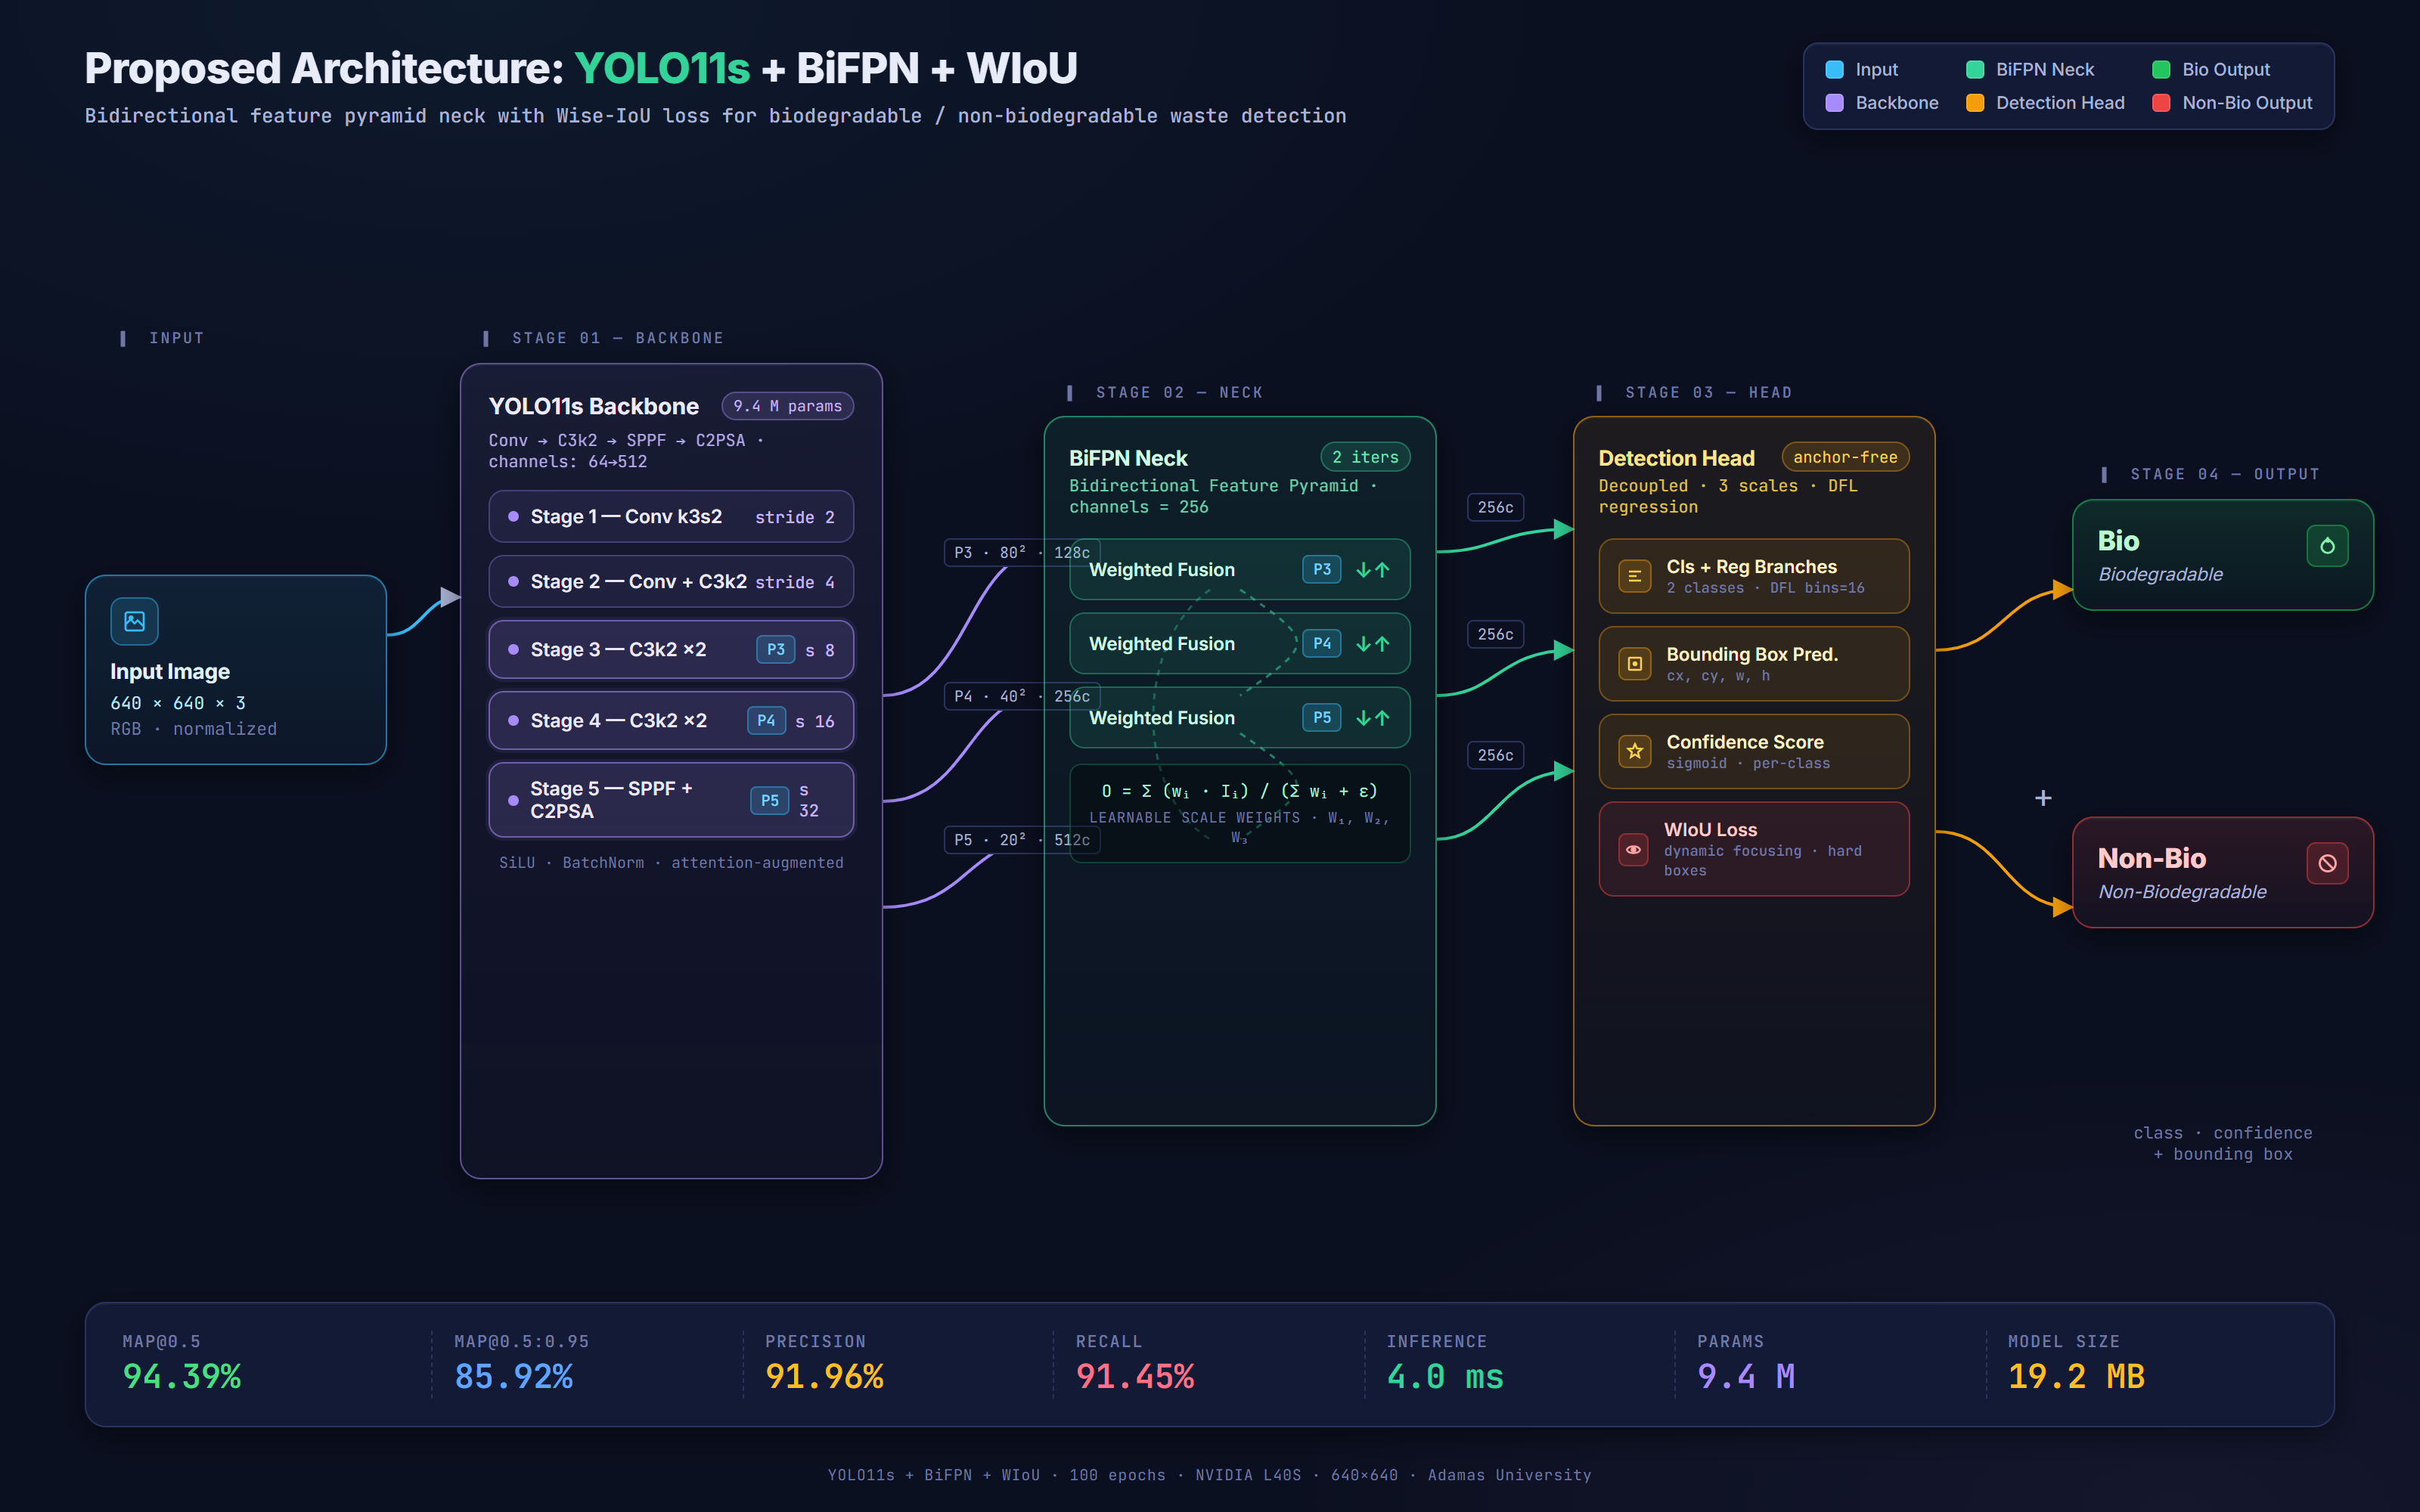
\includegraphics[width=\textwidth]{images/architecture_diagram.png}
    \caption{Proposed System Architecture: YOLO11s + BiFPN + WIoU}
    \label{fig:architecture}
\end{figure}

\section{Key Contributions}

This project makes the following original contributions:

\begin{enumerate}
    \item \textbf{Public Waste Detection Dataset:} A 3,000-image manually annotated dataset covering mixed indoor and outdoor waste scenarios — diverse backgrounds, partial occlusion, fresh and degraded items — expanded to 10,175 images through structured augmentation and released publicly on Roboflow Universe under CC BY 4.0.
    \item \textbf{Systematic Ablation Study:} An eight-step controlled experiment isolating the contribution of each architectural component — the first such study of this scope for binary waste detection, directly addressing a gap identified by recent systematic reviews.
    \item \textbf{Evidence-Based Architecture:} Empirical demonstration that data augmentation (+15.0\% mAP@0.5) dominates all architectural changes combined, and that WIoU v3 with BiFPN provides the best accuracy-complexity trade-off, while CBAM and deformable convolutions degrade performance on this task.
    \item \textbf{High-Performance Model:} Final YOLO11s + BiFPN + WIoU v3 model achieving \textbf{94.39\% mAP@0.5} on the validation set and \textbf{85.46\% mAP@0.5} on the independent held-out test set, at 4.0\,ms GPU inference latency with a 19.2\,MB model footprint.
    \item \textbf{Deployable Demo Application:} A fully functional real-time Streamlit application supporting image upload and webcam detection — addressing the widely noted absence of deployment-ready open systems in the waste classification research community.
\end{enumerate}

\section{Organisation of the Report}

The remainder of this report is organised as follows:

\begin{itemize}
    \item \textbf{Chapter 2 — Literature Review:} Reviews ten existing works in waste classification, IoT-based systems, and YOLO-based detection. Identifies research gaps addressed by this project.
    \item \textbf{Chapter 3 — Technology:} Describes all software frameworks, libraries, and hardware used in this project.
    \item \textbf{Chapter 4 — System Design:} Presents functional and non-functional requirements, system architecture, data flow, and module descriptions.
    \item \textbf{Chapter 5 — Methodology:} Details the dataset construction process, model architecture design decisions, training strategy, and evaluation metrics.
    \item \textbf{Chapter 6 — Implementation:} Describes the practical implementation of each component, including dataset preparation, training code, ablation experiments, and the demo application.
    \item \textbf{Chapter 7 — Results and Analysis:} Presents and analyses all experimental results including the ablation study, final model performance, per-class metrics, and visual outputs.
    \item \textbf{Chapter 8 — Conclusion:} Summarises the project's achievements and key findings.
    \item \textbf{Chapter 9 — Future Work:} Proposes directions for extending this work.
\end{itemize}
